% !TEX TS-program = pdflatex
% !TEX encoding = UTF-8 Unicode

% This is a simple template for a LaTeX document using the "article" class.
% See "book", "report", "letter" for other types of document.

\documentclass[11pt]{article} % use larger type; default would be 10pt

\usepackage[utf8]{inputenc} % set input encoding (not needed with XeLaTeX)

%%% Examples of Article customizations
% These packages are optional, depending whether you want the features they provide.
% See the LaTeX Companion or other references for full information.

%%% PAGE DIMENSIONS
\usepackage{geometry} % to change the page dimensions
\geometry{a4paper,margin=0.5in} % or letterpaper (US) or a5paper or....
 %\geometry{margins=2in}{a4paper} % for example, change the margins to 2 inches all round
% \geometry{landscape} % set up the page for landscape
%   read geometry.pdf for detailed page layout information

\usepackage{graphicx} % support the \includegraphics command and options

% \usepackage[parfill]{parskip} % Activate to begin paragraphs with an empty line rather than an indent
\usepackage{graphicx}
\usepackage{caption}
\usepackage{color} 
\usepackage{epstopdf}
\usepackage{rotating}
\usepackage{lscape}
\usepackage{lineno}
\usepackage{multirow}
%%% PACKAGES
\usepackage{amsmath} 
\usepackage[table]{xcolor}
\usepackage{breakcites}
\usepackage{amsfonts}
\usepackage{booktabs} % for much better looking tables
\usepackage{array} % for better arrays (eg matrices) in maths
\usepackage{paralist} % very flexible & customisable lists (eg. enumerate/itemize, etc.)
\usepackage{verbatim} % adds environment for commenting out blocks of text & for better verbatim
\usepackage{subfig}
% make it possible to include more than one captioned figure/table in a single float
% These packages are all incorporated in the memoir class to one degree or another...
\usepackage{bm}
%%% HEADERS & FOOTERS
\usepackage{fancyhdr} % This should be set AFTER setting up the page geometry

\usepackage{authblk}

\pagestyle{fancy} % options: empty , plain , fancy
\renewcommand{\headrulewidth}{0pt} % customise the layout...
\lhead{}\chead{}\rhead{}
\lfoot{}\cfoot{\thepage}\rfoot{}

%%% SECTION TITLE APPEARANCE
\usepackage{sectsty}
\allsectionsfont{\sffamily\mdseries\upshape} % (See the fntguide.pdf for font help)
% (This matches ConTeXt defaults)

%%% ToC (table of contents) APPEARANCE
\usepackage[nottoc,notlof,notlot]{tocbibind} % Put the bibliography in the ToC
\usepackage[titles,subfigure]{tocloft} % Alter the style of the Table of Contents
\renewcommand{\cftsecfont}{\rmfamily\mdseries\upshape}
\renewcommand{\cftsecpagefont}{\rmfamily\mdseries\upshape} % No bold!
%%% END Article customizations

%%% The "real" document content comes below...

\title{Supervised Learning in Spiking Neural Networks with FORCE Training} 


\date{\today} % Activate to display a given date or no date (if empty),
         % otherwise the current date is printed 
\author[1]{Wilten Nicola}
\author[1]{Claudia Clopath \thanks{c.clopath@imperial.ac.uk}}
\affil[1]{Department of Bioengineering, Imperial College London.  Royal School of Mines\\ London  UK\\  SW7 2AZ}

\begin{document}
\maketitle    


\section*{Acceptance} Note that this manuscript has been accepted and published as of Dec 20th, 
2017 in Nature Communications.  Please cite the following when referencing this manuscript: 


\textbf{
Nicola, W., \& Clopath, C. (2017). Supervised learning in spiking neural networks with FORCE training. Nature communications, 8(1), 2208.}


\section*{Abstract}

Populations of neurons display an extraordinary diversity in the behaviors they affect and display. 
Machine learning techniques have recently emerged that allow us to create networks of model neurons 
that display behaviours of similar complexity. Here, we demonstrate the direct applicability of one 
such technique, the FORCE method, to spiking neural networks.  We train these networks to mimic 
dynamical systems, classify inputs, and store discrete sequences that correspond to the notes of a song. 
Finally, we use FORCE training to create two biologically motivated model circuits. One is inspired by the  
zebra-finch and successfully reproduces songbird singing. The second network is motivated by the hippocampus 
and is trained to store and replay a movie scene.   
FORCE trained networks reproduce behaviors comparable in complexity to their inspired circuits and 
yield information not easily obtainable with other techniques such as behavioral responses to 
pharmacological manipulations and spike timing statistics.  

\section*{Introduction}  

Human beings can naturally learn to perform a wide variety of tasks  quickly and efficiently.  
Examples include learning the complicated sequence of motions in order to take a slap-shot in Hockey or 
learning to replay the notes of a song after music class.   
While there are approaches to solving these different problems in fields such as machine learning, 
control theory, etc., humans use a very distinct tool to solve these problems: the spiking neural network.  


\section*{Results} 



\subsubsection*{FORCE Trained Rate Networks Learn Using Chaos} 

To demonstrate the basic principle of this method and to compare with our spiking network simulations, 
we applied FORCE training to a network of rate equations (Figure \ref{FORCE1}A) as in \cite{FORCE1}.  
We trained a network to learn a simple 5 Hz sinusoidal oscillator.  

\subsection*{High-Dimensional Temporal Signals Improve FORCE Training}

We were surprised at how robust the performance of the songbird network was given 
the high dimensionality and complicated structure of the output.  
We hypothesized that the performance of this network was strongly associated to the precise, 
clock-like inputs provided by HVC and that similar inputs could aid in the encoding and 
replay of other types of information.  To test this hypothesis, we removed the HVC input pattern 
and found that the replay of the learned song was destroyed (not shown), 
similar to experimental lesioning of this area in adult canaries \cite{nottebohm}.   
Due to the temporal information that these high-dimensional signals provide, 
we will subsequently refer to them as High-Dimensional Temporal Signals 
(HDTS, See Materials and Methods for further details).   



\section*{Discussion} 

We have shown that FORCE training can take initially chaotic networks of 
spiking neurons and use them to mimic the natural tasks and functions demonstrated 
by populations of neurons.  For example, these networks were trained to learn 
low-dimensional dynamical systems such as oscillators which are at the heart of 
generating both rhythmic and non rhythmic motion.   
We found FORCE training to be robust to the spiking model employed, 
initial network states, and synaptic connection types.   

Additionally, we showed that we could train spiking networks to display behaviors 
beyond low dimensional dynamics by altering the supervisor used to train the network.  
For example, we trained a statistical classifier with a network of Izhikevich neurons 
that could discriminate its inputs.  
Extending the notion of an oscillator even further allowed us to store a complicated 
sequence in the form of the notes of a song, reproduce the singing behavior of songbirds, 
and encode and replay a movie scene. 
These tasks are aided by the inclusion of a high-dimensional temporal signal (HDTS) 
that discretizes time by segregating the neurons into assemblies.  
 



\renewcommand{\abstractname}{Acknowledgements}
\begin{abstract}
This work was funded by a Canadian National Sciences and 
Engineering Research Council (NSERC) Post-doctoral Fellowship, 
by the Wellcome Trust (200790/Z/16/Z), the Leverhulme Trust (RPG-2015-171) 
and the BBSRC (BB/N013956/1 and BB/N019008/1).  
We would like to thank Frances Skinner, Chris Eliasmith, Larry Abbott, 
Raoul-Martin Memmesheimer, Brian DePasquale and Dean Buonomano for their comments.  
Finally, we would like to especially thank the anonymous referees.  
Their comments and suggestions greatly improved this manuscript. 
\end{abstract}

\renewcommand{\abstractname}{Conflict of Interest} 
\begin{abstract}
There is no conflict of interest to declare.   
\end{abstract}

\renewcommand{\abstractname}{Author Contributions}
\begin{abstract}
WN performed wrote software and performed simualtions.  
Investigation and analysis was performend by WN and CC.  
WN and CC wrote the manuscript.   
\end{abstract}


\renewcommand{\abstractname}{Data Availability Statement}
\begin{abstract}
The code used for this paper can be found on modelDB (\cite{modeldb}), 
under accession number 190565.
\end{abstract}

\section*{Methods} 
\subsection*{Rate Equations} 

The network of rate equations is given by the following:
\begin{eqnarray}
\tau_s\dot{s}_i &=& -s_i + G\sum_{j=1}^N \omega^0_{ij} r_j + Q\eta_i \hat{x}\\
r_j &=& \begin{cases} F \sqrt{s_j} & s_j\geq 0 \\ 0 & s_j <0   \end{cases} \\
\hat{x}(t) &=& \sum_{j=1}^N \phi_j r_j(t) 
\end{eqnarray} 
where $\omega^0_{ij} $ is the sparse and static weight matrix that induces 
chaos in the network by having $\omega^0_{ij}$ drawn from a normal distribution 
with mean 0 and variance $(Np)^{-1}$, where $p$ is the degree of sparsity 
in the network.  The variables $s$ can be thought of as neuronal 
currents with a postsynaptic filtering time constant of $\tau_s$.   
The encoding variables $\eta_i$ are drawn from a uniform distribution 
over $[-1,1]$ and set the neurons encoding preference over the phase space 
of $x(t)$, the target dynamics.  The quantities $G$ and $Q$ are constants 
that scale the static weight matrix and feedback term, respectively.   
The firing rates are given by $r_j$ and correspond to the Type-I normal form for firing.  
The variable $F$ scales the firing rates.    
The decoders, $\phi_j$ are determined by the Recursive Least Mean Squares (RLS) technique, 
iteratively.  RLS is described in greater detail in the next section.  
For Supplementary Fig. 8 and Supplementary Fig. 9, 
we also implemented the $tanh(x)$ continuous variable equations 
from \cite{FORCE1} for comparison purposes.  
These equations are described in greater detail in \cite{FORCE1}.  
 



\subsection*{Integrate-and-Fire Networks} 
Our networks consist of coupled integrate-and-fire neurons, 
that are one of the following three forms: 
\begin{eqnarray}
\dot{\theta}_i &=& (1-\cos(\theta_i)) +\pi^2 (1+\cos(\theta_i))( I)  \quad \text{(Theta neuron)}\\
\tau_m\dot{v}_i &=& -v_i + I  \quad \text{(LIF Neuron)} \\
C\dot{v}_i &=& k(v_i-v_r)(v_i-v_t) - u_i +I  \quad \text{(Izhikevich Neuron)} \\
\dot{u}_i &=& a(b(v_i -v_r) - u_i) 
\end{eqnarray}

The currents, $I$ are given by $I=I_{Bias}+ s_i$ where $I_{Bias}$ is a constant background current 
set near or at the rheobase (threshold to spiking) value.   
The currents are dimensionless in the case of the theta neuron while dimensional for the LIF and Izhikevich models.  
Note that we have absorbed a unit resistance into the current for the LIF model.   
The quantities $\theta_i$, or $v_i$ are the voltage variables while $u_i$ is the 
adaptation current for the Izhikevich model.  
These voltage variables are instantly set to a reset potential ($v_{reset}$) when a 
neurons membrane potential reaches a threshold ($v_{thr}$,LIF) or voltage peak 
($v_{peak}$, theta model, Izhikevich model).  The parameters for the neuron models 
can be found in Table \ref{Table1}.  The parameters from the Izhikevich model are from 
with a slight modification to the $k$ parameter.  The LIF model has a refractory time period, 
$\tau_{ref}$ where the neuron cannot spike.      
The adaptation current, $u_i$ for the Izhikevich model increases by a discrete amount 
$d$ every time neuron $i$ fires a spike and serves to slow down the firing rate.  
The membrane time constant for the LIF model is given by $\tau_m$.  
The variables for the Izhikevich model include $C$ (membrane capacitance), 
$v_r$ (resting membrane potential), $v_t$ (membrane threshold potential), 
$a$ (reciprocal of the adaptation time constant), 
$k$ (controls action potential half-width) and $b$ (controls resonance properties of the model).  

The spikes are filtered by specific synapse types.  
For example, the single exponential synaptic filter is given by the following:
\begin{eqnarray}
\dot{r}_j = -\frac{r_j}{\tau_s} + \frac{1}{\tau_s}\sum_{t_{jk}<t}\delta(t-t_{jk})  \label{fr11}
\end{eqnarray}
where $\tau_s$ is the synaptic time constant for the filter and $t_{jk}$ 
is the $k$th spike fired by the $j$th neuron.  
The double exponential filter is given by 
\begin{eqnarray}
\dot{r}_j &=& -\frac{r_j}{\tau_d} + h_j \\
\dot{h}_j&=& -\frac{h_j}{\tau_r} + \frac{1}{\tau_r\tau_d} \sum_{t_{jk}<t}\delta(t-t_{jk})  \label{fr12}
\end{eqnarray}
where $\tau_r$ is the synaptic rise time, and $\tau_d$ is the synaptic decay time.    
The filters can be of the simple exponential type, double exponential, 
or alpha synapse type ($\tau_r = \tau_d$).   
However, we will primarily consider the double exponential filter with a rise time of 
2 ms and a decay time of 20 ms.  
Longer and shorter filters are considered in the Supplementary Materials.   

The synaptic currents, $s_i(t)$, are given by the equation 
\begin{eqnarray}
s_i = \sum_{j=1}^N  \omega_{ij}r_j 
\end{eqnarray} 
The matrix $\omega_{ij}$ is the matrix of synaptic connections and controls 
the magnitude of the postsynaptic currents arriving at neuron $i$ from neuron $j$.  

 The primary goal of the network is to approximate the dynamics of an 
$m$-dimensional teaching signal, $\bm x(t)$, with the following approximant:
\begin{eqnarray}
\hat{\bm{x}}(t) = \sum_{j=1}^N \bm \phi_j r_j
\end{eqnarray}
where $\bm \phi_j$ is a quantity that is commonly referred to as the 
linear decoder for the firing rate.   
The FORCE method decomposes the weight matrix into a static component, 
and a learned decoder $ \bm{\phi}$:
\begin{eqnarray}
\omega_{ij} = G \omega^0_{ij} + Q \bm{\eta}_i \cdot \bm{\phi}_j  ^T
\end{eqnarray}
The sparse matrix $\omega_{ij}^0$ is the static weight matrix that induces chaos.  
It is drawn from a normal distribution with mean $0$, and variance $(Np^2)^{-1}$, 
where $p$ is the sparsity of the matrix.  Additionally, the sample mean for 
these weight matrices was explicitly set to $0$ for the LIF and theta neuron 
models to counterbalance the resulting firing rate heterogeneity.  
This was not necessary with the Izhikevich model.   
The variable $G$ controls the chaotic behavior and its value varies from 
neuron model to neuron model.   The encoding variables, $\bm \eta_i$ are 
drawn randomly and uniformly from $[-1,1]^k$, where $k$ is the dimensionality of 
the teaching signal.  The encoders, $\bm \eta_i$, contribute to the tuning 
preferences of the neurons in the network.  The variable $Q$ is increased 
to better allow the desired recurrent dynamics to tame the chaos present in the reservoir.    
The weights are determined dynamically through time by minimizing 
the squared error between the approximant and intended dynamics, 
$\bm{e}(t) = \hat{\bm{x}}(t) -\bm{x}(t)$.  
The Recursive Least Squares (RLS) technique updates the decoders accordingly:
\begin{eqnarray}
\bm{\phi}(t) &=& \bm{\phi}(t-\Delta t) - \bm{e}(t)\bm{P}(t)\bm{r}(t) \label{eq14} \\
\bm{P}(t) &=& \bm{P}(t-\Delta t) -\frac{ \bm{P}(t-\Delta t) \bm{r}(t)\bm{r}(t)^T \bm{P}(t-\Delta t)}{1 + \bm{r}(t)^T \bm{P}(t-\Delta t) \bm{r}(t)} \label{eq15}
\end{eqnarray} 
where $\bm{P}(t)$ is the network estimate for the inverse of the correlation matrix:
\begin{eqnarray}
\bm{P}(t)^{-1} = \int_{0}^t \bm r(t) \bm r(t)^T \,dt + \lambda I_N .
\end{eqnarray}
The parameter $\lambda$ acts both as a regularization parameter \cite{haykin} 
and controls the rate of the error reduction while $I_N$ is an $N\times N$ identity matrix.  
The RLS technique can be seen to minimize the squared error between 
the target dynamics and the network approximant:
\begin{eqnarray}
C = \int_0^T(\hat{x}(t)-x(t))^2\,dt + \lambda \bm{\phi}^T \bm{\phi}  
\end{eqnarray}
and uses network generated correlations optimally by using the correlation matrix $P(t)$.  
The network is initialized with $\bm{\phi}(0) = \bm 0$, $\bm P(0) = I_N\lambda^{-1}$, 
where $I_N$ is an $N$-dimensional identity matrix.  
Note that in the original implementation of \cite{FORCE1}, 
equation (\ref{eq14}) contains the term $1+\bm r(t)^T \bm P(t-\Delta t) \bm r(t)$ in the denominator.  
This term adds a slight increase in accuracy and stability, but does not change 
the overall order of convergence of RLS.  
For comparison purposes, this modification was applied to Supplementary Fig. 8.  
All other implementations used equations (\ref{eq14})-(\ref{eq15}).   


\subsection*{High Dimensional Temporal Signals} 

The High-Dimensional Temporal Signals (HDTS) serves to stabilize 
network dynamics by organizing the neurons into assemblies.  
These assemblies fire at precise intervals of time.   
To elaborate further, these signals are constructed as a 
discretization of time, $T$ into $m$ sub-intervals.   
Each subinterval generates an extra component (dimension) in the supervisor 
and within the subinterval, a pulse or upward deflection of the 
supervisor is generated.  For example, if we consider the interval 
from $[0,T]$ with $m$ subintervals of width 
$I_n = [T\left(\frac{n-1}{m}\right),T\left(\frac{n}{m}\right)]$, $n=1,2,\ldots m$.  
The supervisor is constructed as a series of pulses centered in the intervals $I_n$.  
This can be done in multiple ways.  For example, Gaussian pulses 
can be used to construct the HDTS:
\begin{eqnarray}
x_n(t) = \exp\left(-\frac{\left(t - T\left(\frac{2n-1}{2m} \right)\right)^2}{\sigma^2} \right)
\end{eqnarray}
where $\sigma$ controls the width.  Alternatively, 
one can also use piecewise defined functions such as
\begin{eqnarray}
x_n(t) = \begin{cases} |\sin(\frac{m\pi t}{T})| & t\in I_n\\ 0 & \text{otherwise}. \end{cases}
\end{eqnarray}
The end effect of these signals is to divide the network into a series of assemblies.  
A neurons participation in the $n$th assembly is a function of the static weight matrix, 
in addition to $\bm \eta_{in}$.  Each assembly is activated by the preceding assemblies 
to propagate a long signal through the network.  The assemblies are activated at a specific 
frequency in the network, dictated by the width of the pulses in the HDTS.  
Sinusoidal HDTS were used for the all figures with the exception of Supplementary 
Fig. 18C, where a Gaussian HDTS was used.    



\subsection*{The FORCE Method with Rate Networks (Figure 1) }
A network of rate equations is used to learn the dynamics of a teaching signal, $x(t)$, 
a 5 Hz sinusoidal oscillation.  The network consists of 1000 rate neurons with $F = 10$, 
$\tau_s = 10$ ms, $G=1$, and $Q=1.5$, $p=0.1$.    
The network is run for 1 second initially, with RLS run for the next 4 seconds, 
and shut off at the 5 second mark.  The network is subsequently run for another 5 seconds 
to ensure learning occurs.   The smooth firing rates of the network were less than 30 Hz.  
The RLS parameters were taken to be $\Delta t = 2$ ms and $\lambda^{-1} =  0.5$ ms.  



\newpage

\begin{figure}[htp!]
\centering 
\end{figure}


\begin{figure}[htp!]
\centering
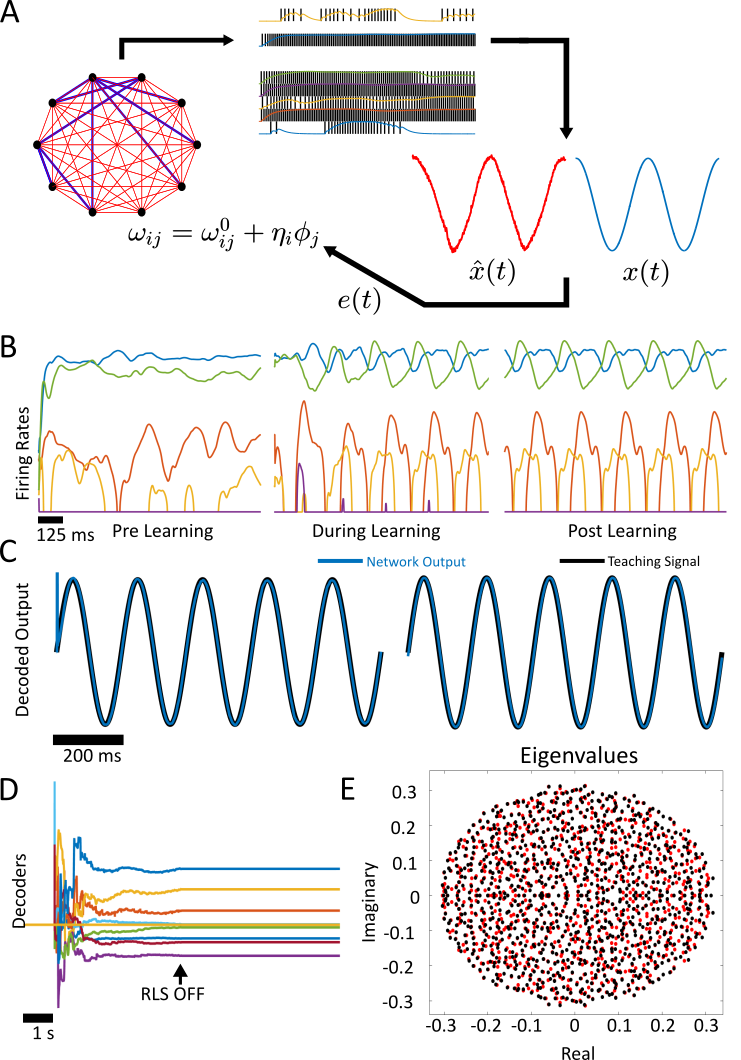
\includegraphics[scale=0.8]{FFIG1}
\caption{}\label{FORCE1}
\end{figure}


\begin{table}[htp!]
\center
\begin{tabular}{|l|l|l|}
\hline 
Neuron Model & Parameter & Value \\
\hline
Izhikevich & $C$ & 250 $\mu$ F  \\ 
\hline
& $v_r$ & -60 mV \\ 
\hline
& $v_{t}$ & -20 mV( -40 mV songbird example, -19.2 mV Supplementary Oscillator Panel) \\ 
\hline
& $b$ & 0  (-2 nS in Supplementary Oscillator Panel)\\ 
\hline
& $v_{peak}$ & 30 mV \\ 
\hline
& $v_{reset}$ & -65 mV \\ 
\hline
& $a$ & 0.01 ms$^{-1}$ (0.002 ms$^{-1}$, songbird example) \\ 
\hline
& $d$ & 200 pA (100 pA, songbird example) \\ 
\hline
& $I_{Bias}$ & 1000 pA \\
\hline
& $k$ & 2.5 nS  \\
\hline
& $\tau_R$ & 2 ms\\
\hline
&  $\tau_D$ & 20 ms \\
\hline 
Theta Model & $I_{Bias}$ & 0 \\
\hline
 & $\tau_R$  & 2 ms \\
\hline 
& $\tau_D $  & 20 ms\\
\hline 
LIF Model &$\tau_m$ & 10 ms  \\
\hline 
& $\tau_{ref}$ & 2 ms  \\ 
\hline 
&$v_{reset}$ & -65 mV  \\
\hline 
& $v_{t}$ & -40 mV \\ 
\hline 
& $I_{Bias}$& -40 pA (-39 pA, Lorenz Example) \\
\hline 
\end{tabular}
\caption{The parameters used for the Izhikevich, theta, and LIF neuron models, unless otherwise stated} \label{Table1} 
\end{table}



\newpage 
\section*{Figure Captions} 



\subsection*{Figure \ref{FORCE1}:  The FORCE Method Explained  }
(A) In the FORCE method, a spiking neural network contains a backbone of static 
and strong synaptic weights that scale like $1/\sqrt{N}$ to induce network level chaos (blue).  
A secondary set of weights are added to the weight matrix with the decoders 
determined through a time optimization procedure (red).  
The Recursive Least Squares technique (RLS) is used in all subsequent simulations.  
FORCE training requires a supervisor $x(t)$ to estimate with $\hat{x}(t)$. 
(B) Prior to learning, the firing rates for 5 random neurons from a network of 1000  
rate equations are in the chaotic regime.  The chaos is controlled and converted 
to steady state oscillations. (C)  This allows the network to represent a 5 Hz 
sinusoidal input (black). After learning, the network (blue) still displays the 
5 Hz sinusoidal oscillation as its macroscopic dynamics and the training is successful. 
The total training time is 5 seconds.  (D) The decoders for 20 randomly selected neurons 
in the network, before ($t<5$), during ( $5\leq t<10$) and after ($t\geq 10$) 
FORCE training.   (E) The eigenvalue spectrum for the effective weight matrix 
before (red) and after (black) FORCE training.  
Note the lack of dominant eigenvalues in the weight matrix.  



\newpage
\bibliographystyle{apalike}	% or "unsrt", "alpha", "abbrv", etc.

\bibliography{references}






\end{document}
